\documentclass[preprint]{sigplanconf}
\usepackage{cleveref,amsmath,chngcntr}
\usepackage{textcomp} % for tilde
\usepackage{paralist} % for in-paragraph lists
\usepackage{url}
\usepackage{graphicx}

% For drawing FSMs
%\usepackage{tikz}
%\usetikzlibrary{arrows,automata}

% Used for code snippets
\usepackage{listings,courier}
\usepackage{subfig,epsfig}
\DeclareCaptionType{copyrightbox}
\usepackage{epsfig}


% Settings on code listings.
\lstset{language=C,
		xleftmargin=0pt,
		xrightmargin=0pt,
		framexbottommargin=0pt,
        framextopmargin=0pt,
        framesep=0pt}
\usepackage{enumitem}

% Add listing language for assembly
\lstdefinelanguage
   [x64]{Assembler}     % add a "x64" dialect of Assembler
   [x86masm]{Assembler} % based on the "x86masm" dialect
   % with these extra keywords:
   {morekeywords={CDQE,CQO,CMPSQ,CMPXCHG16B,JRCXZ,LODSQ,MOVSXD, %
                  POPFQ,PUSHFQ,SCASQ,STOSQ,IRETQ,RDTSCP,SWAPGS, %
                  rax,rdx,rcx,rbx,rsi,rdi,rsp,rbp, %
                  r8,r8d,r8w,r8b,r9,r9d,r9w,r9b}} % etc.

% For leaving some comments in the draft.
\newcommand{\comment}[1]{}

% Customize cleverref
\crefname{section}{Section}{Sections}

\begin{document}

%make title bold and 14 pt font (Latex default is non-bold, 16 pt)
\title{Granary: A Sane Framework for Instrumenting an Insane Environment}

%for single author (just remove % characters)
\authorinfo{Peter Goodman \and Akshay Kumar \and Angela Demke Brown \and Ashvin Goel}
{University of Toronto}{}
% end authorinfo

\maketitle
\subsection*{Abstract}
Kernel modules extend the functionality of operating systems. They represent the bulk of new kernel code in development and contain the majority of new kernel bugs. Unfortunately, analysing and debugging modules is very challenging. Static analysis of module source code is difficult because of the tight interaction between modules and the kernel. Some modules, however, are only distributed in a binary format, which makes static analysis intractable. Existing dynamic analysis tools capable of instrumenting modules are not suited toward module analysis. They either impose unnecessary performance overheads, lack flexibility and are too coarse-grained, or do not provide a means of understanding the ``big picture'' view of what an arbitrary module does as it executes.

We created Granary to address the challenges of module analysis. Granary is a framework for creating flexible and efficient tools that analyse or debug arbitrary, binary Linux kernel modules. Granary uses dynamic binary translation to dynamically rewrite and comprehensively instrument kernel modules. Granary makes it easy to create flexible tools by supporting context-aware runtime code specialisation, and by integrating high-level static analysis information with low-level instruction manipulation. Module analysis tools built on Granary are efficient because of Granary's adoption of a relaxed transparency model, and because of Granary's ability to instrument module code without imposing overhead on non-module kernel code.


\section{Introduction}\label{sec:intro}

Operating system (OS) kernels present an apparently insane environment for a transparent binary instrumentation framework.  For example, hardware interrupts can redirect control flow at any instruction, and interrupt delivery cannot be delayed past the execution of memory instructions that might alter the interrupt delivery state~\cite{DRK}. Preserving interrupt transparency, however, requires that interrupts be delayed until the end of any injected instrumentation instructions.  Together, these requirements make it very difficult to write instrumentation tools.  The insane environment of OS kernels also creates several opportunities for analysis tools. For example, interrupts can be ``tamed'' and put to new uses; privileged hardware features can be used; and the kernel ABI and source code can be relied upon to be a good predictor of module behaviour at the kernel/module boundary. We also found that the kernel is largely insensitive to transparency issues, allowing us to relax transparency in exchange for both improved performance and greater visibility into the execution of instrumented code.  This increased visibility is particularly important for analysis and debugging tools.

The challenges and opportunities of the kernel environment motivated the creation of Granary. Granary is a new binary instrumentation framework for the Linux kernel environment, designed specifically for analysing kernel modules. Granary targets modules because they represent the bulk of new bugs and new code in development in the Linux kernel \cite{FaultsInLinux}. Granary allows developers to create flexible and dynamic analysis tools for arbitrary Linux kernel module binaries. Granary has two main goals: \begin{inparaenum}[i)]
	\item make it easy to create efficient, low-level analysis tools; and
	\item provide high-level static analysis information to the analysis tools.
\end{inparaenum} Granary achieves the first goal by using dynamic binary translation (DBT) to provide low-level access to instructions, memory, and interrupts. Granary achieves the second goal by giving tools direct access to the results of its own static analysis of the Linux kernel source code. By meeting these goals, Granary tools are able to do things like  figure out which data structure fields are associated with each memory access.

Granary addresses three limitations of existing program analysis systems: \begin{inparaenum}[i)]
	\item they have focused on instrumenting all code (the whole kernel: DRK; or whole system: QEMU, PinOS);
	\item they do not allow for flexible runtime code specialisation (Pin, DynamoRIO); and
	\item they do not provide static type information to the instrumented code (Pin, DynamoRIO).
\end{inparaenum} 

Instrumenting all code (e.g., the whole kernel) imposes unnecessary performance overheads when only a subset of the code is being analysed (e.g., modules). In practice, we would like to target instrumentation at specific modules for efficiency, while also allowing rich and detailed instrumentation of these modules and any other relevant code. This requirement motivates the design of \emph{mixed-mode execution}, which allows Granary to instrument module code while non-module kernel code executes with zero overhead. This is challenging because Granary must be comprehensive: all code that is meant to be instrumented should be instrumented. In other words, relinquishing control to execute kernel code natively must not cause Granary to miss the execution of any module code.

Another limitation of existing systems is that they are unable to perform efficient runtime code specialisation, i.e. they are unable to change how code is instrumented based on the context in which that code will run. For example, Granary has a tool that  dynamically constructs inter- and intra-procedural control flow graphs (CFGs). The outputs of this tool enable Granary to do better runtime register allocation, which improves tool efficiency. Part of building CFGs requires tracking whether or not a given basic block is the entrypoint to a function. This is challenging with existing DBT systems because some optimised functions will re-execute their first basic block, which might incorrectly appear as new function calls in the CFGs. Granary solves this problem using demand-based runtime code specialisation: every entrypoint basic block is instrumented in one way, and later re-executions of any entrypoint basic blocks are specialised and instrumented in another way.

In Granary, code is specialised according to the context in which that code will execute. In the previous example, executing code is classified into two contexts: entrypoint and non-entrypoint basic blocks. Granary tracks execution contexts using a technique we call \emph{policy-driven instrumentation}. In a Granary tool, each tracked execution context is associated with its own instrumentation policy. An instrumentation policy decides how to instrument code that will execute within the associated context. In the case of our CFG tool, two policies track the two execution contexts: $P_{\mathit{call\_entry}}$ and $P_{\mathit{after\_entry}}$. $P_{\mathit{call\_entry}}$ applies to the first execution of the first basic block of each function, and connects functions in the inter-procedural CFG.  $P_{\mathit{after\_entry}}$ applies to all other executed basic blocks within each function, including re-executions of the first basic block. $P_{\mathit{after\_entry}}$ connects basic blocks in the intra-procedural CFG. Granary is able to track execution contexts because it explicitly maintains policy information in translated basic blocks. This avoids typical problems with tracking context in just-in-time DBT systems (e.g., concurrency, arbitrary pre-emption, context-switch\-ing, inability to predict later execution contexts at translation time).

Finally, an important missing feature of existing low-level instrumentation systems is the ``big picture'' view that one gets from static analysis information. Similarly, static analysis tools lack access to instructions, memory, and processor-specific behaviours that are only available to low-level runtime instrumentation tools. Existing mixed static/dynamic analysis tools \cite{NaCl,AddressSanitizer,ThreadSanitizer} appear to get the best of both worlds, but sacrifice on runtime flexibility by committing to a single instrumentation policy at a program's compile time. The benefits of high-level static analysis motivated its inclusion into Granary using a technique we call \emph{reifying instrumentation}. Granary statically analyses the Linux kernel source code to bootstrap learning about  the interfaces that enable modules and the kernel to interact. Granary exposes this information to instrumentation tools in the form of type and function \emph{wrappers}. Tools can use wrappers to apply context-specific policies when instrumenting module code as well as to inspect and manipulate parts of kernel/module memory in a type-safe way.

For example, we are actively developing a tool that uses static type information to learn about all the fields of all kernel data structures that are read from or written to by modules. This information allows us to model things like how a typical file system operates on kernel data structures in the process of opening a file. From these models, we can construct behavioural patterns about how modules use kernel data structures and functions. These patterns can be used to classify modules \cite{DeviceDriverClassification} and identify spurious behaviour \cite{LXFI}.

The rest of the paper describes Granary in more detail. \Cref{sec:modes} describes how to efficiently implement mixed-mode execution. \Cref{sec:policies} describes a new method for dynamically changing how code is instrumented. \Cref{sec:reify} describes how to integrate static analysis information into a DBT system. Finally, \Cref{sec:eval} evaluates Granary's performance.

\section{Dynamic Binary Translation}\label{sec:dbt}

Granary uses dynamic binary translation (DBT) to instrument Linux kernel modules. DBT is used for instruction set translation/emulation \cite{QEMU}, runtime optimization \cite{DynamoRIOOptimisation}, and runtime instrumentation (analysis \cite{DynamoRIO}, security \cite{Vx32,NaCl}, and debugging \cite{Valgrind}). We chose DBT because \begin{inparaenum}[i)]
	\item static binary analysis tools are unable to cope with \texttt{x86}'s mix of variably-sized instructions and data; 
	\item some modules are only distributed in a binary format; and
	\item virtualisation-based approaches are unable to analyse non-virtualisable device drivers \cite{DRK}.
\end{inparaenum}

Granary interposes on the Linux kernel's module loading process. When a kernel module is loaded, Granary bootstraps by translating the first basic block of the module's initialisation function.  It then replaces the pointer to that function with a pointer to the translated basic block. The translation process continues when the kernel initialises the module by invoking the translated module code.

Granary translates and instruments module binaries one basic block at a time. That is, new basic blocks are decoded and translated as execution ``discovers'' those basic blocks. Translated basic blocks are linked together and stored in a globally accessible \emph{code cache}. In Granary, a basic block is a sequence of instructions ending in a conditional branch, \texttt{ret}, or \texttt{jmp}, but not a \texttt{call} instruction.

Granary's just-in-time translation approach means that code executing from the code cache may yield control to Granary to request the address of the next basic block to execute. When instrumented code yields to Granary, a ``context switch'' occurs that transfers execution to a CPU-private stack where Granary operates. Granary context-switches back to the code cache when the next basic block has been found or translated so that instrumented execution may continue. Similar to other DBT systems, Granary uses caching and hotpatching to reduce the number of context switches. In our experience, modules stabilise very quickly: context switches stop happening after most module basic blocks have been translated.

Basic blocks in Granary's code cache contain \texttt{x86-64} binary instructions and meta-data describing those instructions. The meta-data that Granary records in each basic block includes: \begin{inparaenum}[i)]
	\item the length in bytes of the original and translated basic blocks;
	\item the address of the first instruction in the original basic block; and
	\item the policy information (e.g., $P_{\mathit{call\_entry}}$, $P_{\mathit{after\_entry}}$) used to instrument the basic block.
\end{inparaenum} This meta-data can be queried and extended by Granary instrumentation tools. For example, Granary's CFG-building tool represents each node in the inter- and intra-procedural CFGs as an extension of the meta-data stored for each basic block. The meta-data is also queried by interrupt handlers when deciding how to handle interrupts in instrumented code, and by debuggers (e.g., \texttt{gdb}) to give contextual information about a translated basic block. 

%\begin{figure*}[t!]
%\lstset{language=C, tabsize=2, stepnumber=1}
%\begin{multicols}{2}
%\begin{lstlisting}[basicstyle=\footnotesize\ttfamily]
%struct device_driver {
%	...
%	int (*probe)(struct device *);
%	int (*remove)(struct device *);
%	void (*shutdown)(struct device *);
%	int (*suspend)(struct device *, pm_message_t);
%	int (*resume)(struct device *);
%	...
%	const struct dev_pm_ops *pm;
%	...
%};
%\end{lstlisting}
%\columnbreak
%\begin{lstlisting}[basicstyle=\footnotesize\ttfamily]
%TYPE_WRAPPER(struct device_driver, {
%    PRE_OUT {
%        ABORT_IF_FUNCTION_IS_WRAPPED(arg.probe)
%        WRAP_FUNCTION(arg.probe);
%        WRAP_FUNCTION(arg.remove);
%        ...
%    }
%    POST_OUT {
%        POST_WRAP(arg.pm);
%    }
%})
%\end{lstlisting}
%\end{multicols}
%\vspace{-1em}
%\caption{The Linux device driver structure is shown on the left. The automatically generated type wrapper for this structure is shown on the right. In the wrapper code, \texttt{arg} is a reference to a \texttt{struct device\_driver} object passed as, or referenced by, an argument to a kernel or module wrapper. Code in the \texttt{PRE\_OUT} section is applied to arguments of the wrapped type before a kernel wrapper is invoked. Similarly, code in the \texttt{POST\_OUT} section is applied to arguments of the wrapped type after a kernel wrapper is invoked. \texttt{POST\_WRAP} invokes the type wrapper that is specific to the value to which it is applied (\texttt{arg.pm}). Type wrappers also support \texttt{\_IN} suffixes instead of \texttt{\_OUT} suffixes, which apply to data going into modules (i.e., over module wrappers). Finally, the \texttt{RETURN\_} prefix is used to apply some code to return values of either kernel or module wrappers.}
%\label{fig:type_wrapper}
%\end{figure*}

\section{Mixed-Mode Execution}\label{sec:modes}
Granary supports two modes of execution: instrumented and native. Module code is instrumented and executes from Granary's code cache, which is under Granary's control. Non-module kernel code runs natively. A mode switch occurs when execution transfers between native and instrumented code. Some mode switches happen naturally (e.g., when instrumented code returns to native code) and other mode switches are mediated by Granary (e.g., when instrumented module code invokes a kernel function).

The mode switch from instrumented module code to native kernel code is easier to detect since the instrumented code runs under Granary's control. Granary treats all kernel functions as \emph{detach} points, where a mode switch from instrumented to native code occurs. At these points, Granary stops executing.

However, Granary needs a way to regain control when native kernel code invokes module code. Our fallback solution for regaining control uses hardware page protection to trap attempts by the kernel to execute native module code. We handle these traps by redirecting execution to instrumented module code. While comprehensive, this approach is not ideal because: \begin{inparaenum}[i)]
	\item trapping on every execution attempt introduces overhead; and
	\item the trap does not provide sufficient information about which interfaces were being used by the kernel to invoke the module.
\end{inparaenum}

Granary's main approach to regaining control is based on the observation that modules tell the kernel about their interfaces by registering functions with the kernel. We expect that at least some of the registered functions will be executed by the kernel because this is the mechanism by which modules extend the kernel's functionality. To Granary, registered module functions represent potential future \emph{attach} points, where a mode switch from native to instrumented code will occur. Furthermore, Granary discovers additional attach points at detach points by observing pointers to module functions that are passed by modules to the kernel.

Granary uses static analysis to dynamically discover attach points by wrapping the kernel/module interface. Kernel functions are wrapped by \emph{kernel wrappers} that inspect and traverse argument pointers in search of pointers to module functions. \Cref{fig:type_wrapper} shows an example of a type wrapper for the Linux device driver structure. If a pointer to a module function (a future attach point) is discovered, then Granary replaces that pointer with a function-specific \emph{module wrapper}. Granary inspects and modifies arguments to module wrappers in the same way as for kernel wrappers. This allows Granary to discover kernel entry points that will cause instrumentation to detach. Finally, Granary redirects execution to the appropriate kernel or instrumented module function after wrapping has occurred.

Kernel and module wrappers invoke \emph{type wrappers} to find and wrap pointers to module functions that are directly or indirectly referenced by kernel/module function arguments. A type wrapper is a function that recursively  traverses the in-memory object graph and converts pointers to module code into pointers to wrapped module functions. Type and kernel wrappers are automatically generated at Granary's compile time by scripts that statically analyse the kernel source code. Granary automatically matches any variable in a kernel wrapper to a type wrapper if the base type (absent pointers, specifiers, and qualifiers) of that variable matches the type wrapper's wrapped type. Similarly, Granary automatically generates module wrappers using a combination of compile-time meta-programming and runtime code generation to match type wrappers to the declared arguments of \texttt{C} function pointer types.  Granary's wrapper approach has two benefits: (i) it is more efficient than the trap-based alternative, and (ii) it gives instrumentation tools more information about the executing module (\Cref{sec:reify}).

After Granary bootstraps on the module initialisation process, \emph{attaching} occurs in one of three ways: \begin{enumerate}
	\item {\bf Implicit attaching:} the kernel returns to instrumented module code in the code cache.
	\item {\bf Fast attaching:} the kernel invokes a wrapped module function.
	\item {\bf Slow attaching:} the kernel invokes unwrapped module code. If the kernel executes a module function which was passed to the kernel in a type-unsafe manner, then the processor will raise a fault because Granary uses hardware page protection to prevent module code from being executed. Granary handles these faults by returning execution to the instrumented version of the faulting module code.
\end{enumerate}

Granary \emph{detaches} when control transfers from instrumented code to native (uninstrumented) code. Detaching occurs in one of two ways: \begin{enumerate}
	\item {\bf Implicit detaching:} instrumented module code returns to the original kernel, or is interrupted (initial interrupt handling is done by the kernel).
	\item {\bf Wrapped detaching:} instrumented module code invokes a kernel wrapper, which later transfers control to the kernel.
\end{enumerate}


\subsection{Transparency}\label{sec:transparency}

An instrumentation system is transparent if, given the same inputs, the instrumented and uninstrumented versions of a program behave in the same way \cite{Transparency}. Granary includes configurable levels of transparency to address the trade-off between transparency and overhead. By default, Granary uses a relaxed transparency model for efficiency, flexibility and increased visibility, but if instrumentation for some module requires transparency then it can be enabled at the cost of increased overheads and decreased visibility. By default, Granary exposes the following three artifacts: code cache addresses as function and interrupt return addresses, and wrapped module function addresses in shared data structures.

\vspace{-3pt}\paragraph{Function return addresses}\label{para:return_address_transparency} Unlike most DBT frameworks, Granary defaults to inlining \texttt{call} instructions into basic blocks, which exposes code cache addresses to instrumented module code in the form of return addresses. Inlining \texttt{call} instructions avoids return-address mispredictions and unnecessary control-flow by building longer basic blocks. If Granary is configured to use transparent return addresses, then implicit attaching and detaching are disabled because they depend directly on returning to instrumented module or native kernel code. Granary will fall back to slow attaching to handle kernel-to-module returns, and indirect branch lookups for module-to-module returns.

\vspace{-3pt}\paragraph{Interrupt return addresses} Kernel interrupts are not sensitive to return addresses and hence relaxing return address transparency has no effect on interrupts. A special case arises for page fault exceptions that occur within specific kernel functions that access user space data. Granary handles this special case in a similar way to the kernel. Thus, maintaining return address transparency with respect to interrupts in instrumented module code has no value.

\vspace{-3pt}\paragraph{Module function wrappers} Granary does not maintain transparency when its type wrappers replace pointers to module functions with pointers to wrapped module functions. This is perhaps the riskiest break in transparency within Granary because a module might treat a function pointer as being representative of the module being in some particular state.\footnote{We have not yet encountered a module where changing pointers to module functions into module wrappers altered the module's behaviour under instrumentation.} If Granary is configured to use transparent module function pointer addresses in shared data structures then fast attaching is disabled and tools will not have access to the same level of static program information.


%\lstset{language=[x64]Assembler}
%\newsavebox\asmbox
%\begin{lrbox}{\asmbox}
%\begin{minipage}[b]{4cm}
%\begin{lstlisting}[basicstyle=\footnotesize\ttfamily]
%1: mov    (%rdi), %rax
%   jmp    2
%2: mov    %rax, (%rsi)
%   test   %rax
%   jz     4
%3: inc    %rsi
%   inc    %rdi
%   jmp    1
%4: ret
%\end{lstlisting}
%\end{minipage}
%\end{lrbox}
%
%\begin{figure*}[ht!]
%\vspace{-2em}
%\centering
%\subfloat[Policy Switching Protocol]{
%\begin{tikzpicture}[>=stealth',shorten >=1pt,auto,node distance=3cm,scale=0.8, every node/.style={scale=0.8}]
%  \node[initial,state]          (C)   {$P_{\mathit{call\_entry}}$}; 
%  \node[state]          (A)[right of=C]      {$P_{\mathit{after\_entry}}$};
%  \path[->]     (A)     edge    [loop above]    node {{\footnotesize\ttfamily\bf jmp}, {\footnotesize\ttfamily\bf jz}} (A)                                edge         [bend right]        node {{\footnotesize\ttfamily\bf call}} (C)                        (C) edge    [bend right]     node {{\footnotesize\ttfamily\bf jmp}, {\footnotesize\ttfamily\bf jz}} (A)                        (C)     edge    [loop above]    node {{\footnotesize\ttfamily\bf call}} (C);
%\end{tikzpicture}
%}
%\hfill
% \subfloat[Uninstrumented Code]{\usebox\asmbox}
%\hfill
% \subfloat[Instrumented Basic Blocks]{
%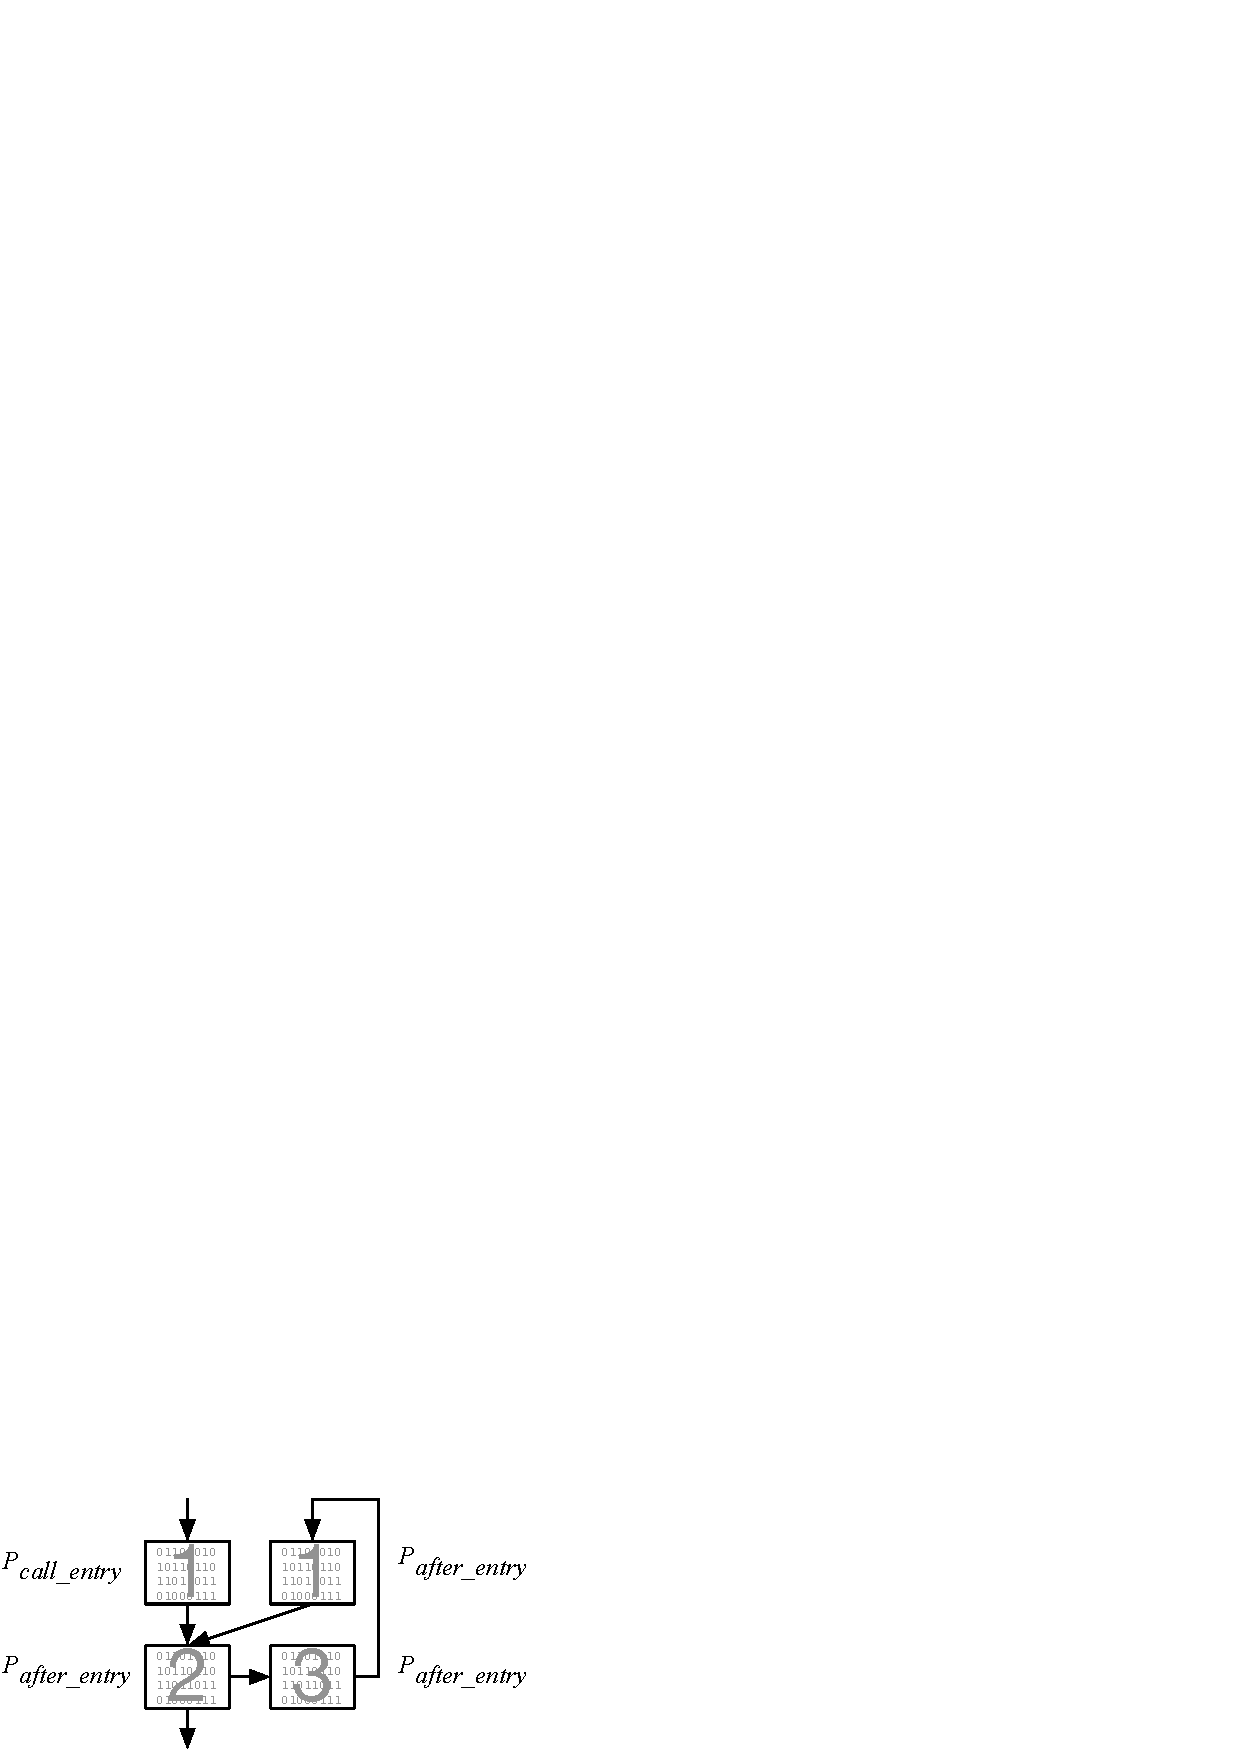
\includegraphics[width=2.5in]{diagrams/policy-switching-entry-tracking.pdf}
% }
%\ORIGcaption{\label{fig:policy_switching}Example policy switching protocol that ensures that instrumentation ($P_{\mathit{call\_entry}}$) is performed only once on entry to every function, regardless of if that basic block is re-executed by a non-\texttt{call} instruction. Basic block (1) is instrumented by both $P_{\mathit{call\_entry}}$ and $P_{\mathit{after\_entry}}$, and basic blocks (2) and (3) are instrumented by $P_{\mathit{after\_entry}}$.}
%\end{figure*}


\section{Policy-Driven Instrumentation}\label{sec:policies}

A natural extension of mixed-mode execution is to give Granary tools the ability to dynamically switch the policy used to instrument code. Instrumenting only module code allows Granary to specialise the execution of native code. In the same way, policy switching allows tools to specialise the execution of instrumented code. In fact, optimising the performance of an early Granary tool was the original motivation for policy switching.

We developed a Granary tool that detects several Read-Copy-Update (RCU) API misuses in module code. Our tool focused on read-side critical sections (delimited by calls to \texttt{rcu\_read\_lock} and \texttt{rcu\_read\_unlock} in the code), however, most code executes outside of read-side critical sections. As an optimisation, we wanted our heavyweight API-checking instrumentation to apply only when the code was executing within a read-side critical section. Implementing this optimisation was challenging because each basic block was only translated once, and we had no way to know whether or not the heavyweight instrumentation should be applied to it. Knowing the state (within or outside a read-side critical section) at translation time was not sufficient, since the same translated block could later be executed in the opposite context. That is, code executing \emph{within} a read-side critical section may have originally been translated while executing \emph{outside} of a read-side critical section, and would thus omit the heavyweight API-checking instrumentation. This omission could cause our tool to miss bugs (i.e., it would not be comprehensive) when the basic block executes within a read-side critical section.

To implement this optimisation, Granary enables tailoring instrumentation to the context in which the instrumented code will execute. To do so, Granary allows different versions of the same module code to co-exist within Granary's code cache. That is, a different version of each of a module's basic blocks exists in Granary's code cache  for each encountered execution context. In the case of our RCU checker tool, there were two execution contexts: within and outside of a read-side critical section. If the same module basic block is  executed in the two contexts, then Granary's code cache would contain two different instrumented versions of that basic block. The way that Granary distinguishes between different execution contexts is with \emph{instrumentation policies}. 

An instrumentation policy is both a name for an execution context, as well as a function that decides how to instrument basic blocks that will execute within that context. All tools define an initial policy that Granary uses to instrument module code. Tools are not limited to one policy though: any policy can declare a policy switch that will take effect when a selected control-transferring instruction (CTI) is executed. For example, our RCU tool invokes a policy switch from policy $P_{\mathit{null}}$ to policy $P_{\mathit{read\_critical}}$ when $P_{\mathit{null}}$'s instrumentation function observes a \texttt{call} instruction to the \texttt{rcu\_read\_lock} Linux kernel function.

Because policies name an execution context, they also represent states in a finite state machine. That is, a module's execution is in the state named by a policy if the code executing was instrumented by that policy. A state transition occurs when control transfers from code instrumented by one policy to code instrumented by another policy. A limitation with this approach is that a single state does not encode the sequence of previous states that led to execution being in the current state. For example, RCU permits nested read-side critical sections. If two read-side critical sections are nested then switching from $P_{\mathit{read\_critical}}$ to $P_{\mathit{null}}$ on the first \texttt{call} to \texttt{rcu\_read\_unlock} meant that our tool would lose track of being in the context of the outer read-side critical section. We solved this limitation by observing that, in most cases, function returns are natural policy reverting points. This is because the runtime call stack encodes both the context in which the current code is executing, as well as the continuation of the current executing code.

The effect of a tool specifying a policy switch on a CTI is that the basic block(s) targeted by that CTI will be instrumented according to the specified policy. CTIs with unspecified policies inherit their policies from their containing basic blocks. As hinted at above, \texttt{ret} instructions cannot explicitly switch policies, which allows a function instrumented by a different policy than its caller to return to the caller's context (i.e., policy). The asymmetry between \texttt{call}s and \texttt{ret}s is intentional: \texttt{call}s place contextual breadcrumbs (in the form of return addresses) on the runtime call stack, and \texttt{ret}s read these breadcrumbs to return to a previous context. Under this lens, the instruction pointer tracks our current policy, and return addresses form a stack of previous policies. Policy switches behave similarly to state transitions in a pushdown automaton; \texttt{call} instructions push a new state onto the stack for each function, \texttt{ret} instructions pop the current function's state from the stack, and other CTIs induce state transitions within the current function by altering control flow.

Granary implements policy tracking and switching by encoding policy information into the meta-data and CTIs of basic blocks. If a policy switch is not specified on an instrumented CTI then that CTI inherits the policy used to instrument the basic block containing the CTI. When an instrumented CTI executes for the first time, it yields control to Granary with the CTI target and policy information as inputs. Granary decodes and instruments the targeted instructions according to the input policy information. Because every non-\texttt{ret} CTI encodes policy information, and because Granary's translation mechanism depends only on CTI policy and target information, Granary is able to ensure that policy information is never lost or corrupted, even in the face of concurrent executions of the same module code, arbitrary pre-emption, and arbitrary resumption.

One example of a tool that uses policy switching is Granary's CFG tool, which dynamically constructs runtime inter- and intra-procedural control-flow graphs (CFGs). A single policy approach for call graph construction might add edges to the call graph only at every \texttt{call} site. However, this approach is insufficient in the face of mixed-mode execution. If an instrumented function $F$ is only invoked by a native function (which contains no instrumentation), and $F$ contains no function calls, then $F$ will not appear as a root node in the call graph. A two-policy solution easily solves the missing root problem by instrumenting both function call sites as well as function entrypoints. The CFG tool distinguishes between the first execution of a function's first basic block ($P_{\mathit{call\_entry}}$), and all other basic blocks executed within the function, including later executions of the first basic block ($P_{\mathit{after\_entry}}$). Function call sites are instrumented to set up the source node of an edge in the call graph. On entry to a function, we identify the current function as either a sink node connected to a source node (instrumented call), or as a root node if no source is present (native call). The distinction between entrypoints and non-entrypoints is achieved with minor bloat: the first basic block appears twice in Granary's code cache, but instrumented by two different policies, as shown in \Cref{fig:policy_switching}.




\section{Reifying Instrumentation}\label{sec:reify}

Granary uses a technique we call \emph{reifying instrumentation} to provide the benefits of high-level static analysis information to dynamic instrumentation tools. Reifying instrumentation bootstraps on Granary's mixed-mode execution approach, which exposes static type information to instrumentation tools. For example, we are actively using type information present in wrappers to create a tool that generates models of typical module behaviour. The wrapper information serves two roles in our tool. First, we use type wrappers to assign type-specific IDs to module-allocated memory that is shared across the module/kernel interface. Type ID assignment is critical because it allows us to match memory reads and writes to specific kernel data structure fields. Second, we use the kernel and module function wrappers to generate call graphs of a module's execution. This call graph models module behaviour (according to the kernel) because we label module code nodes with kernel data structure and function pointer field names (derived from module wrappers). This labelling allows us to generalise across similar modules. For example, code reached by calling the \texttt{ext4\_mount} and \texttt{btrfs\_mount} functions from the \texttt{ext4} and \texttt{btrfs} modules, respectively, are both labelled as \texttt{file\_system\_type::mount}, because the function addresses are stored (and later replaced by module wrappers) in the \texttt{mount} field of a \texttt{file\_system\_type} data structure. The combined records from multiple ``trusted'' modules of the same class (e.g., mature, open-source file systems) will model the behaviour of typical kernel modules. We hope that these models will help us build tools that classify and identify spurious module behaviour. 

\section{Evaluation}\label{sec:eval}

We evaluated Granary by measuring the throughput of common file system operations performed by the \texttt{iozone} file system benchmark running on an \texttt{ext3} file system.
To focus on the CPU overhead of Granary and avoid the disk performance bottleneck, we mounted \texttt{ext3} on a 1 GB Ramdisk.  The benchmarks were run on an otherwise idle desktop equipped with an Intel\textregistered\ Core\texttrademark\ 2 Duo 2.93 GHz CPU with 4GB of RAM.  In our experiment, \texttt{iozone} mounts an \texttt{ext3} file system (which installs two kernel modules: \texttt{ext3} and \texttt{jbd}) and creates two processes (reader and writer) that read from and write to a 480MB file 1KB at a time. 


\Cref{fig:perf} shows the decrease in throughput due to Granary (instrumenting only \texttt{ext3} and \texttt{jbd}), DynamoRIO Kernel (DRK; instrumenting the whole kernel and all modules), and ModifiedDRK (DRK modified to instrument only \texttt{ext3} and \texttt{jbd}, but using strict transparency) relative to native execution.  We run tests both using direct I/O, to bypass the OS buffer cache and force all file system requests to go through the \texttt{ext3}/\texttt{jbd} code, and with the OS buffer cache enabled.  Performance bars are overlaid, not stacked (e.g., buffered reads achieve nearly native throughput with both Granary and ModifiedDRK, so the native bar is covered).  Buffering highlights the benefits of mixed-mode execution: Granary and ModifiedDRK introduce almost no overhead for reads because most file system requests are served from the kernel's buffer cache. Direct requests highlight the impact of Granary's relaxed transparency model, which gives Granary lower overheads than ModifiedDRK.

%\begin{figure}[t!]
%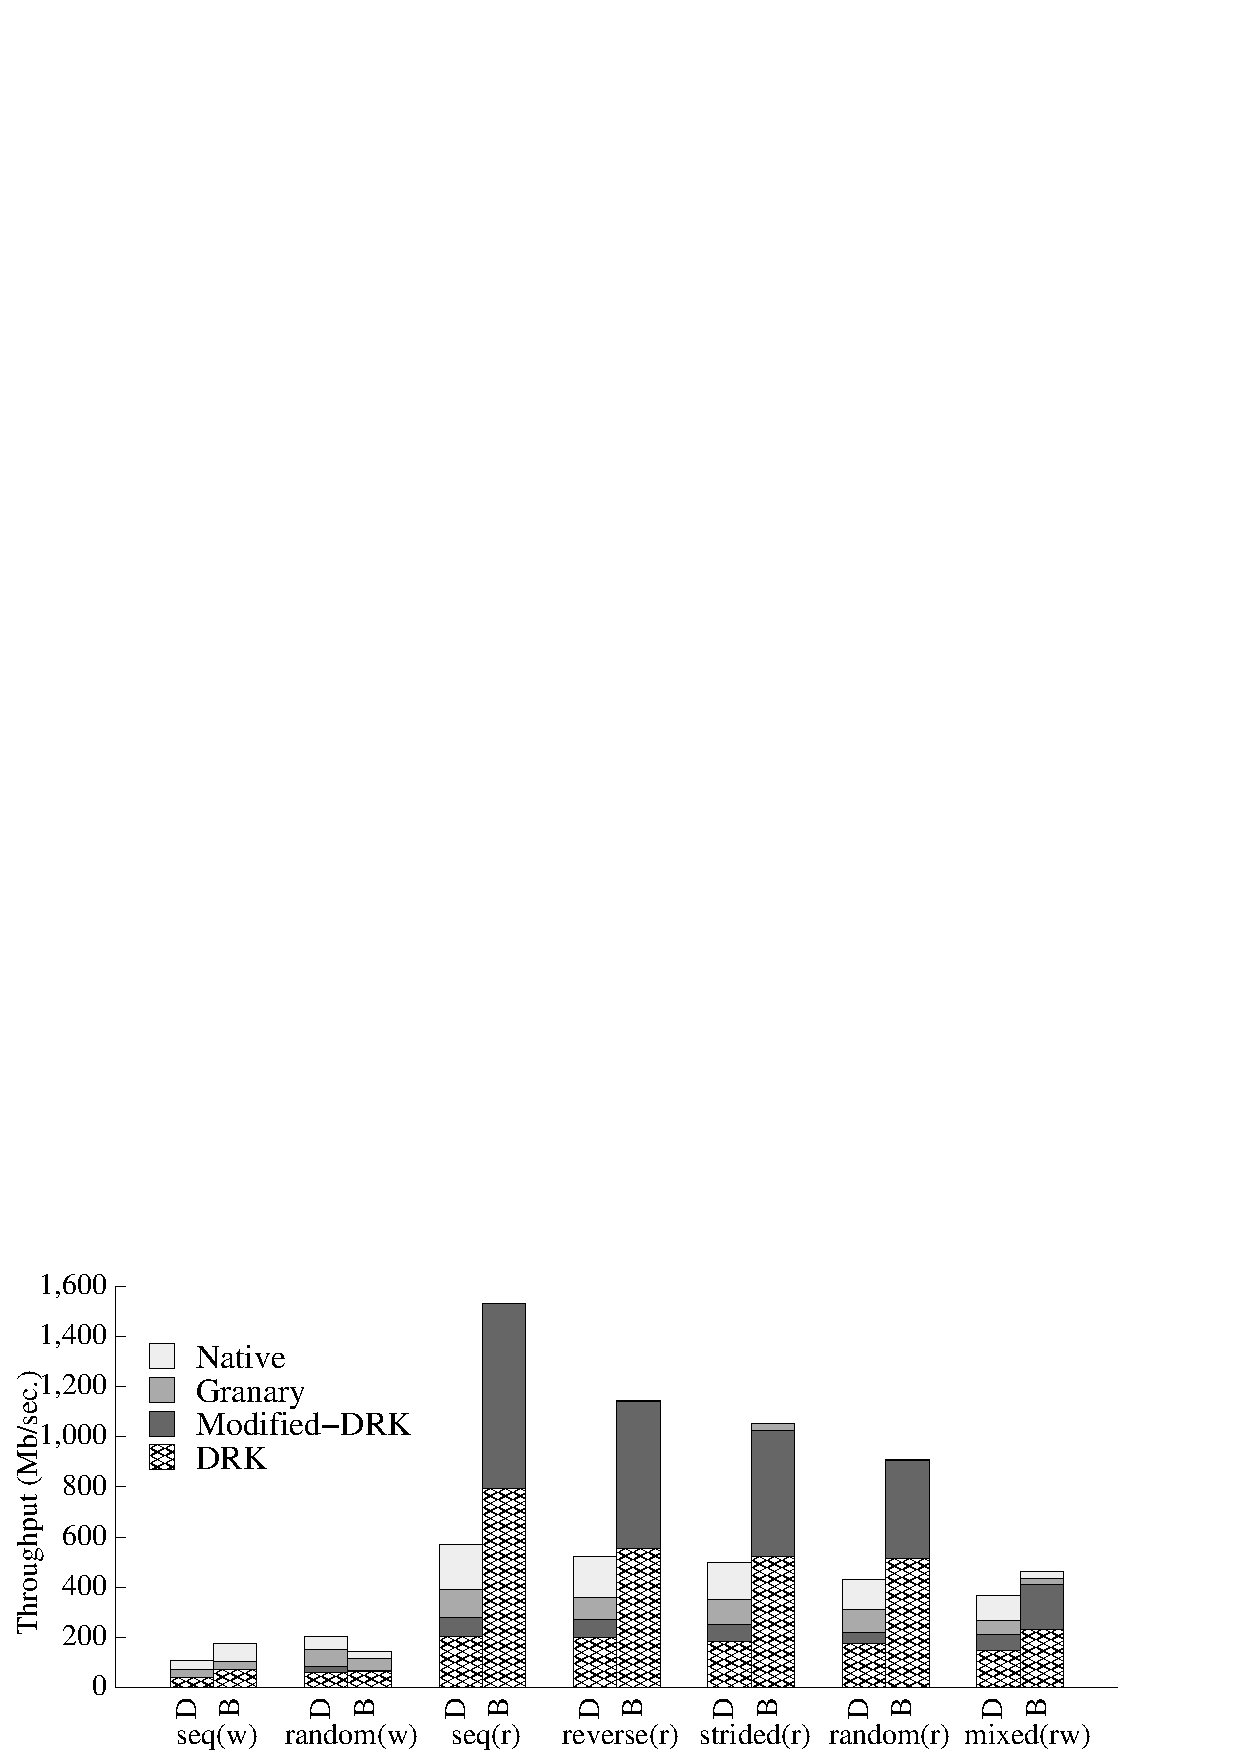
\includegraphics[width=\columnwidth]{diagrams/stacked-performance.pdf}
%\caption{\label{fig:perf}Throughput in MB/sec of common file system operations, for Direct IO (\textbf{D}) where requests bypass the OS buffer cache and Buffered IO (\textbf{B}) where the OS buffer cache is enabled. }
%\end{figure}

\section{Related Work}\label{sec:related}
Prior work can be classified as either whole-kernel/system DBT, or probe-based kernel instrumentation. We discuss how Granary differs from these approaches.
\vspace{-3pt}\paragraph{Whole-kernel/system DBT} DRK \cite{DRK} is a kernel space port of the DynamoRIO \cite{DynamoRIO} DBT framework. DRK instruments the entire kernel, including modules, and follows a strict transparency model, which limits the flexibility of instrumentation and increases overheads.  PinOS \cite{PinOS} is a port of the Pin \cite{Pin} DBT framework that performs whole-system instrumentation. It has high overheads and depends on hardware virtualisation, which prevents it from instrumenting non-virtualisable kernel modules. 

\vspace{-3pt}\paragraph{Probe-based Instrumentation} Several systems support injecting code at specific locations within kernel code. For example, KernInst \cite{KernInst} can inject code at almost any location in an unmodified commodity OS. Other examples with similar or more restricted functionality include LTTng \cite{LTTng}, KProbes \cite{KProbes}, DProbes \cite{DProbes}, and ftrace \cite{ftrace}. These systems are unable to perform fine-grained instrumentation of instructions or memory.


\section{Conclusion}\label{sec:conclusion}
We created Granary to address the challenges of instrumenting binary kernel modules.  Granary provides mixed-mode execution to remove the overheads of DBT for uninstrumented kernel code.  A relaxed transparency model further improves performance and allows greater visibility into the interactions between module and kernel code.  Granary also supports policy-driven instrumentation, which allows tools to specialise their instrumentation based on the context in which code executes.  Finally, Granary exposes high-level static analysis information to dynamic instrumentation tools, making it easy to match low-level memory reads with specific fields in data structures at the source code level. 
Together, Granary's features simplify the development of powerful kernel module analysis tools, while delivering lower overheads than previous kernel dynamic binary instrumentation solutions.

\bibliographystyle{acm}
\bibliography{library}

\end{document}
